\section{Gothenburg Congestion Tax}\label{sec:gothenburg}

\subsection{Implementation\protect\footnote{This history is based on \citet{Borjesson2015} and \citet{Hysing2015b}.}}

The genesis of Gothenburg's pricing system lies in the above-mentioned infrastructure agreement between Stockholm and the national government. Previously, infrastructure in Sweden had been funded nationally, but in 2008 the government directed the infrastructure administration to prioritize co-financing arrangements like Stockholm's when selecting projects for the 2010-2021 transport investment plan. When a draft of the plan came out in spring 2009, leaders from Gothenburg (Sweden's second largest city) lamented that many of their high-priority projects had been left out, and embarked on negotiations with national officials about co-financing. Negotiations proceeded quickly, and in October 2009 the Gothenburg City Council ratified the ``West Swedish Agreement,'' whereby 17 billion SEK in local funds---including 14 billion from road pricing---would be matched by national funds. The Agreement included a 20 billion SEK rail tunnel (the ``Western Link''), a road tunnel, bus lanes and a multi-modal bridge. 

The scheme design and list of projects to fund was rushed, so that the projects could be included in the national investment plan that Parliament passed in April 2010. The lack of process and revelations about the low benefict-cost ratio of the Western Link provoked controversy. In September 2010 voters gave several seats on the City Council to a new anti-pricing party, Vägvalet (``Road Selection''), and in 2012 a petition led the council to schedule a non-binding referendum on pricing for the 2014 elections. Nevertheless,  the Gothenburg Congestion Tax (GCT) launched on January 1st, 2013. The September 2014, the referendum resulted in 57\% of votes cast against pricing, but the Council kept the Tax in order to fulfill Gothenburg's end of the West Swedish Agreement. In January 2015, tolls were raised after early revenues fell short of those needed for the Agreement.

\subsection{Design}

Gothenburg's scheme uses the same technology and design as Stockholm's: cameras identify drivers crossing tolling sites in either direction, and tolls vary by time-of-day (see Fig. \ref{fig:gothenburg-prices}). There is a daily maximum charge of 60 SEK, and the same vehicles are exempt as in Stockholm. Figure \ref{fig:Gothenburg-map} shows the tolling sites form a cordon around downtown Gothenburg, but there are also sites at the \"Alvsborg Bridge (toll site \#11) and along a highway north of the city where congestion would otherwise be severe.

The GCT has the same exemptions as the SCT and is also turned off in July. One feature unique to the GCT is the ``single charge'' or  ``multi-passage'' rule: no matter how many tolling sites a vehicle crosses within 60 minutes, it is charged only once, with the toll being the highest among the possible charges. 

\begin{figure}[ht]
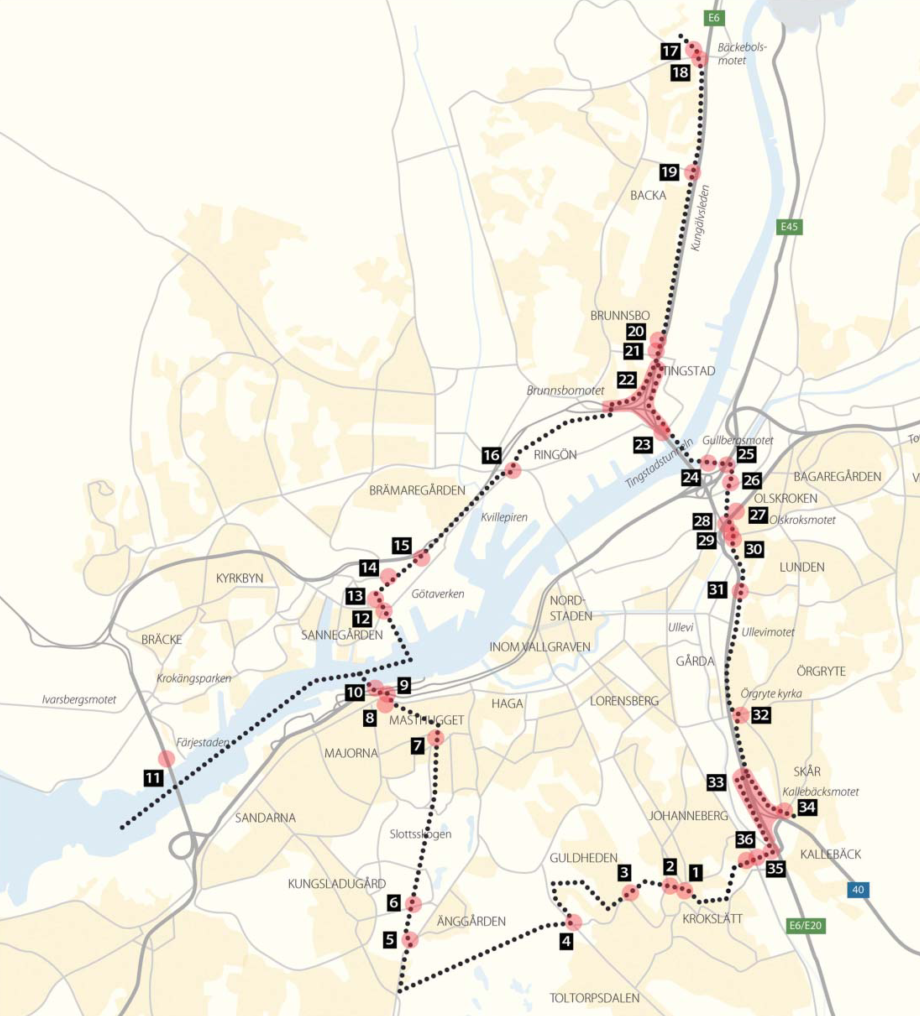
\includegraphics[width=0.7\textwidth]{../img/gburg-map.png}
\caption{Gothenburg Congestion Tax zone \citep{transportstyrelsen2015}\label{fig:Gothenburg-map}}
\end{figure}

\begin{figure}
    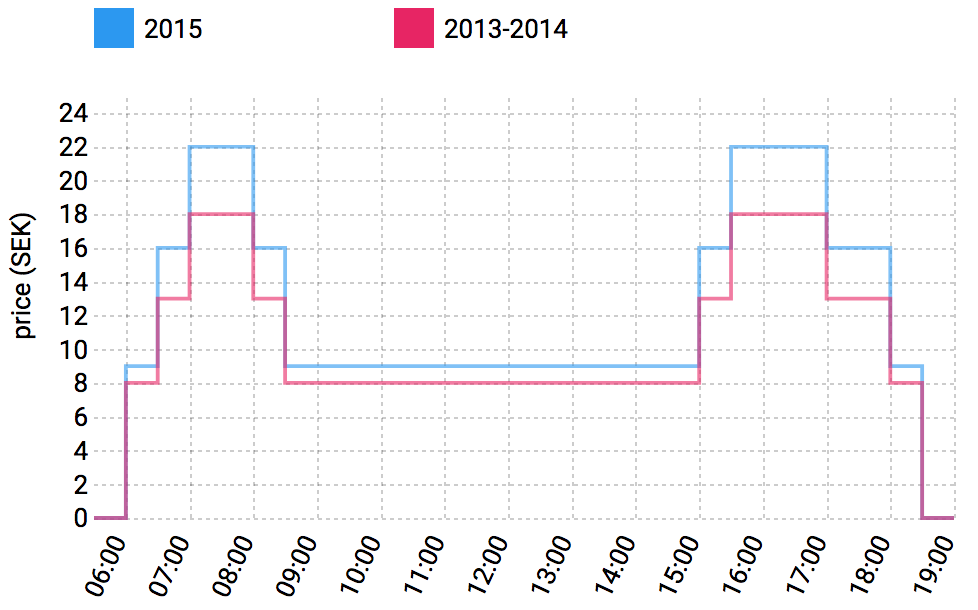
\includegraphics[width=0.8\textwidth]{../img/gothenburg-prices.png}
    \caption{Gothenburg price structure } 
    \label{fig:gothenburg-prices}
\end{figure}

\subsection{Transportation impacts}

Between 2012 and 2013, cordon crossings during charging hours fell 12\%, rather than the 15\% forecast by models \citep{Borjesson2015}. Although peak crossings were expected to fall more than off-peak, due to the higher charges, in fact both fell by about 12-13\%. (Recall that Stockholm also surprised observers by showing the same reduction in the peak and off-peak.) Entries have since remained stable \citet[Tab. 5]{Borjesson2018}.

Travel time savings were mild---mostly because Gothenburg had not been very congested. Results appear in Fig. \ref{fig:Gothenburg-travel-times}. Inner arterials are the highways circled in Fig. \ref{fig:Gothenburg-map}; outer arterials are the uncircled highways outside the zone; bypasses are highways further out than the map shows. The dramatic reduction on the inner arterials is attenuated by the fact that travel time on these links had only been about 5 minutes during the morning peak \citep{Borjesson2015}.

Surveys conducted before and after charging show that commuters switched to public transport, while discretionary travelers traveled less frequently or switched destinations. Accounting for external factors, the charge is estimated to have raised public transport ridership by about 4.5-6.5\% \citep{Borjesson2015}.

\begin{figure}[ht]
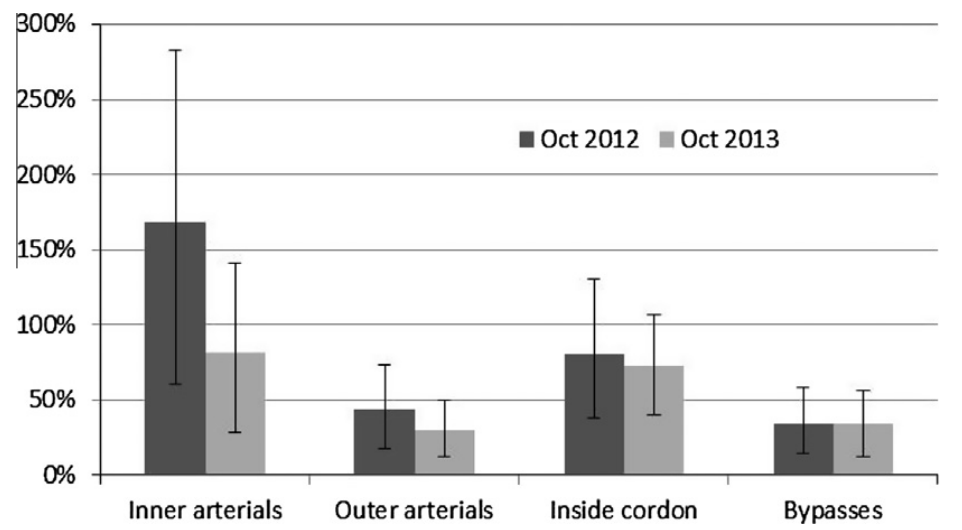
\includegraphics[width=0.55\columnwidth]{../img/gburg-travel-times.png}

\caption{Gothenburg 6-10 A.M. Increase in travel times on selected categories of road relative to free-flow speeds, before (Oct 2012) and after (Oct 2013) the Congestion Tax. \citep{Borjesson2015} \label{fig:Gothenburg-travel-times}}

\end{figure}

Like Stockholm, Gothenburg's experience supports Theme II: the 2015 toll increase resulted in no real change in entries during the peak hours, although the increase was not as substantial as in Stockholm \citep[p. 43, Tab. 6]{Borjesson2018}.

\subsection{Finances}

The GCT cost only 410 MSEK to implement if we count only those costs specific to Gothenburg \citep[p. 40]{Borjesson2018}. However, in 2012, Sweden spent 350 MSEK to replace the IT system for the SCT with a national system used by the GCT and two bridges elsewhere; arguably some part of this expense could be attributed to Gothenburg. 

In the first year, 2013, the GCT earned 720 MSEK in charges and about 80 MSEK in penalties---short of the amount that had been forecast in 2009 \citep[pp. 142-143]{Borjesson2015}. \citet{Borjesson2015} blame the shortfall on economic factors (fuel prices, recession) and the fact that 45\% of trips into the cordon during charging hours took advantage of the ``multi-passage'' rule---rather than the 30\% analysts predicted. The shortfall is what led authorities to raise the toll in 2015, since---unlike in London where revenues are hypothecated to transit in a vague way---the Western Swedish Agreement commits Gothenburg to pay for specific projects. The increase led revenues to jump from 80 MSEK in 2014 to 99.5 million EUR in 2015. Operating costs have been around 130 MSEK per year and are declining \citep[table 3]{Borjesson2018}.




